\documentclass[a4paper]{acm_proc_article-sp}  
\usepackage[utf8]{inputenc}
\usepackage{cmap}
\usepackage{microtype}
\usepackage{mathpazo}
\usepackage{listings}
\usepackage{xspace}
\usepackage{array}
\usepackage{tikz}
\newcommand{\eg}{e.g.\@\xspace}
\newcommand{\ie}{i.e.\@\xspace}
\newcommand{\etc}{etc.\@\xspace}
\newcommand{\Naive}{Na\"{i}ve\@\xspace}
\newcommand{\naive}{na\"{i}ve\@\xspace}
\lstset{language=python,tabsize=2}
\begin{document}

\title{Peer-to-Peer Voting Scheme}
\author{\alignauthor Mitar Milutinovi\'{c} and Valkyrie Savage\\
\affaddr{Computer Science Division\\University of California, Berkeley} \\
\email{mitar@tnode.net valkyrie@eecs.berkeley.edu}\\
\text{CS270 Final Project, Spring 2013}
} 
\maketitle

\setcounter{page}{1}
\pagenumbering{arabic}

\section{Abstract}

We designed a voting scheme which allows a group of people to better decide on a common opinion about an issue. Currently,
the most used approach is to simply count number of votes against and for, while not taking into account people who do
not cast a vote. Our approach is to have each person define delegates whose votes will be counted when he/she does not
vote him/herself. In this way we get a social network, a trust network, between users which can be
used to transitively compute missing votes. We believe such a result better represents the will of the group.

\section{Introduction}

Currently the most common way of a group decision-making is voting with simple vote counting, determining the result by
majority. Such a scheme is easy to understand and implement, but the question is if it does the most important thing
in the best possible way. Namely, the main purpose of a group decision-making scheme is to find the result which would
satisfy the whole group the most. In practice, issues arises because only a small part of the whole group participate
in the decision making, namely by casting a vote. Decisions are thus based on opinions of this smaller part and despite
others not participating in the decision-making they still might have an opinion or a general preference based on their
values, even if they do not know exactly which voting option best satisfies their values. The reason for this is often
lack of the time or knowledge necessary to make an informed decision.

In this paper we address this issue with a novel group decision-making scheme which, when determining the outcome of
the decision-making process, takes into account the social network of the group and relationships between members.
In short, it allows members to delegate their votes to one or more other members. These delegations are used to infer
the missing vote when the member does not vote him- or herself. Such delegations are transitive and form a kind of
social network between members.

The idea falls into the more general idea of proxy voting or voting with delegation.  In the following section we
analyze existing proposals inside this space. After that, we present our proposal in more detail, comparing it with
existing proposals.  We analyze its runtime and data structures.  Finally, we conclude with suggestions for future work.

\section{Related work}

\subsection{Smartocracy}

Smartocracy \cite{smartocracy} is a system implemented by a group of researchers and tested in a beta period with several users from their
institutions.  They implemented a trust-driven social network for decision making along with three different algorithms
for determining which problem solutions were the most desirable by the collective: these three algorithms were direct
democracy, dynamically distributed democracy (DDD), and proxy voting.  Direct democracy is exactly as it sounds;
a person's vote is thrown away if she does not cast a ballot.  DDD allows users to designate a single other person
who is given the power to use their voting influence in the case that they do not cast a ballot.  The proxy voting
algorithm redistributes voting influence based on incoming edges at each node at the beginning of each vote.  That
is, at step 0 everyone receives an equal amount of voting power, then at step 1 voters who are trusted by other
voters are given additional voting influence equal to all the voting influence of the people who trust them.

Vote delegation is transitive such that if Alice does not vote and has delegated her vote to Bob, and Bob does not
vote but has delegated his vote to Cathy, then Cathy has the power to vote with the influence commanded by Alice and Bob.
Delegation is done in general rather than by domain, such that a person who you ``trust'' is implicitly trusted in all
voting situations.

Under all algorithms, solutions voted on by participants can be weighted: e.g. Alice can delegate 40\% of her vote to
solution 1 and 60\% to solution 2.  The solution with the most vote weight at the end of the vote wins.  There is
only a single vote, and no consideration is given to a situation in which there is a cycle of non-voters who trust each other.

\begin{figure}
\centering
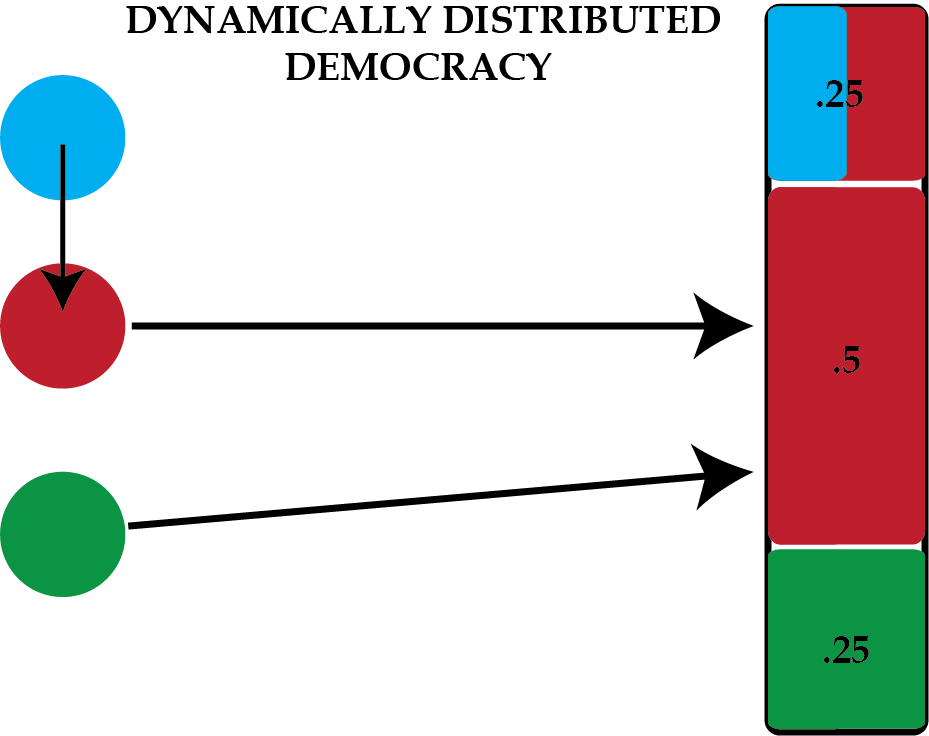
\includegraphics[width=0.45\textwidth]{figures/DDD.png}
\caption{In dynamically distributed democracy, voters are assigned additional voting power at the beginning of a vote, based on how many people trust them.}
\end{figure}

\subsection{Delegative Democracy}

Delegative Democracy \cite{delegative} is an idea, rather than an implemented system, proposed by Bryan Ford.  This system offers voters the
choice of being an active delegate or a passive delegator.  In the first case, they exercise their voting power on their own,
along with any delegated to them.  In the second case, they select one other person to whom they delegate their full voting power.
The system emphasizes exercise of voting strength rather than the current paradigm of winning or losing a seat.  Each person is
initially given the same voting weight, and the final distribution of weights for members of the population depends upon the
trust network.  It is understood that the privacy of non-voting (delegating) individuals is protected by this
system so that they cannot be coerced into giving their vote to particular delegates and that the privacy of voting (delegated)
individuals is waived such that they are held accountable to those whose voting power they hold.

This system offers significant flexibility in delegation.  It is possible to assign votes to different people depending on
which forum the vote is taking place: e.g. votes on environmental policy can be delegated from Alice to Bob, while votes on
space program funding can be delegated from Alice to Cathy.  Delegation is transitive as it propagates through the network.
Cycles in delegation are resolved through delegation ranking.  Alice can state that her votes should go to Bob, but if that is
not possible for some reason (e.g. Bob has delegated his votes to Alice and no one else), Alice can state that her votes go to
Cathy instead.  If ranking does not resolve a cycle, all the voting power of the delegates in the cycle are discarded.  After
delegation resolution, a single majority vote based on voting strength determines the outcome.

\begin{figure}
\centering
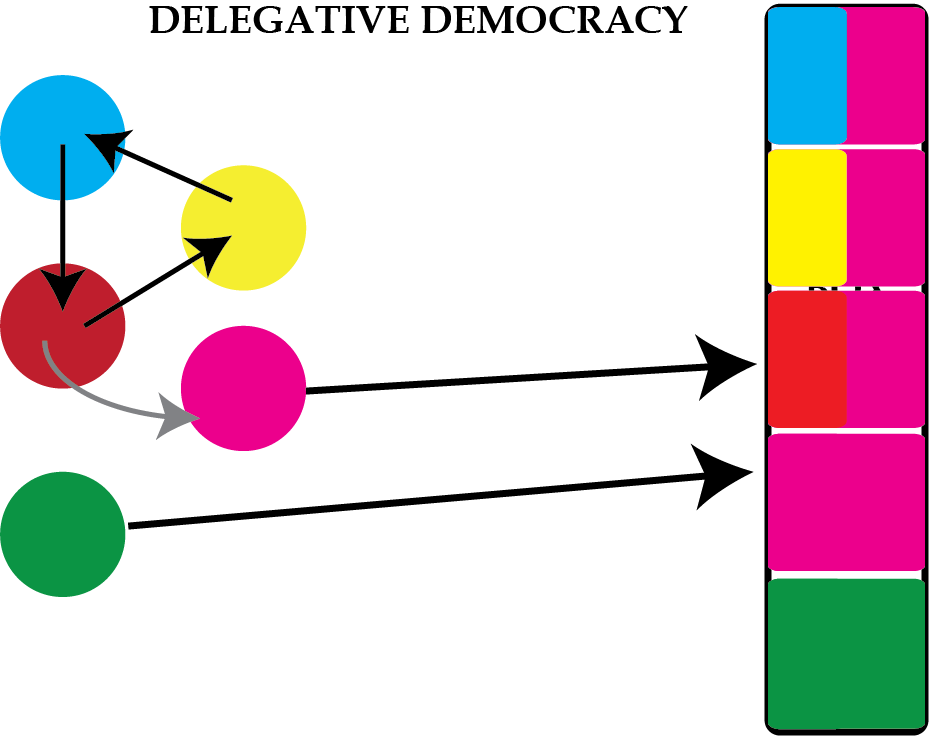
\includegraphics[width=0.45\textwidth]{figures/delegativedemocracy3.png}
\caption{Delegative democracy allows voters to assign delegates of their votes (black lines) and secondary delegates (grey lines) in case of a delegation cycle in which no one casts a vote.}
\end{figure}

\subsection{Toward Delegated Democracy}

The Toward Delegated Democracy paper \cite{tdd} describes two novel methods of determining the outcome of a vote based on a trust-based
social network.  Voters create trust connections to other voters in a multiple transitive delegation system in which voters
delegate their vote to one or many others in general rather than by domain.  The transitive nature of this voting graph is
described by a falloff: i.e. if Alice delegates her vote to Bob and Bob delegates his vote to Cathy, Cathy receives 1 unit of
vote from Bob plus $1 \cdot (1-\mathrm{falloff})$ units of vote from Alice.  This is an attempt to quantify the non-transitive
nature of value systems and trust connections.

All voters are initialized with equal voting power which is distributed through the network based on the trust edges.  Voting
is expected to be performed cyclically; i.e. when a proposal is made, voters vote on it, and as discussion about the proposal
continues, they are free to change their votes.  This is a departure from the traditional voting process and the process
described in all the previous papers.

The real contributions of this paper lie in their outcome estimation algorithms.  Based on the votes of a few voters and the
created trust graph, they can estimate the outcome of the vote.  They also propose a system in which voters who have the most
trust-based voting power and the weakest delegation relations (e.g., if Bob and Cathy have the most voting power of anyone else,
we do not select them both if Bob delegates his power to Cathy) are selected from the social graph and asked to vote: based on
the selection mechanism, they are supposed to be the best representatives of the whole voter community.

\begin{figure}
\centering
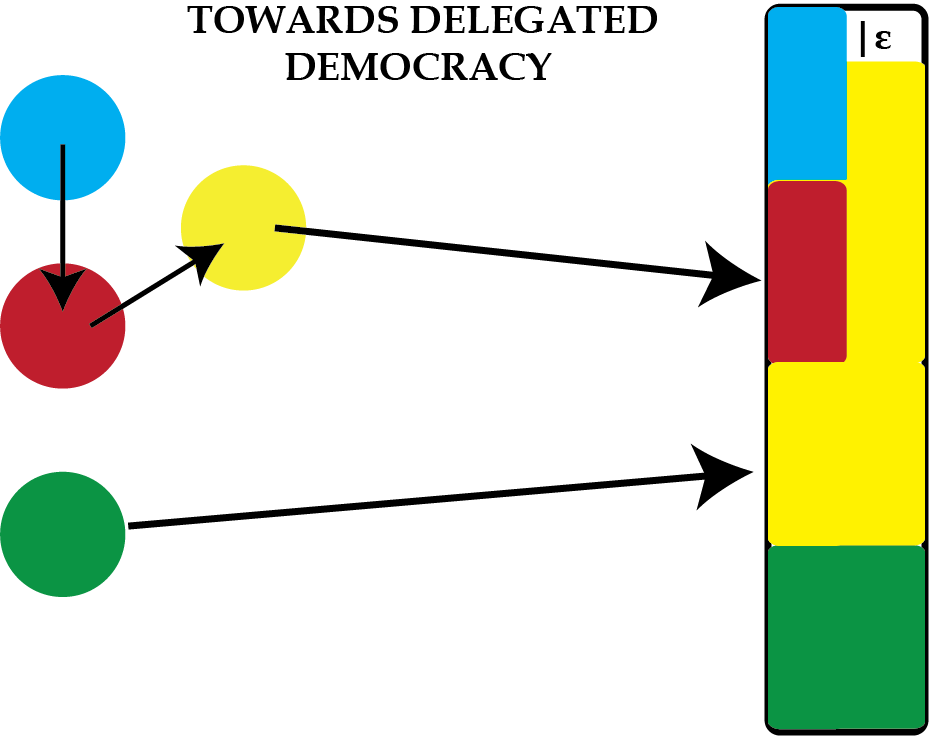
\includegraphics[width=0.45\textwidth]{figures/tdd0.png}
\caption{The Towards Delegated Democracy paper describes the non-transitive nature of trust, in which only 1-$\epsilon$ of the blue vote is transferred from the red delegate to the yellow delegate.}
\end{figure}

\subsection{A Voting System for Internet-Based Democracy (Liquid Democracy)}

Liquid Democracy \cite{liquiddem} focuses on an iterative voting system in which voters can change their votes at any time in order to show
their approval or disapproval of an idea or policy.  This system is based upon a social game (i.e., the prisoner's dilemma)
in which voters identify themselves as part of the group or not.  Voting is performed with transitive delegation (which is
domain-insensitive), but is resolved as a series of voting vectors.  A person has a total of $+1$ voting power, but can
assign $-1$ or $+1$ to all measures being voted upon (such that the sum of all votes totals to $+1$), and the voting is
arbitrated in order to ensure maximum happiness for the group based upon all voting vectors.  Since voting is continuous,
voters can ``vote together'' to improve the strength of their combined vectors and achieve a more preferred outcome.  This
is conducted per the Internet Voting System where voters' voting vectors are represented in n-dimensional space and match up
with points on an n-sphere.  The vectors are added in the usual fashion and the outcomes are determined by their sum.

The main advantage of this system is that it was implemented into multiple software solutions and it is used actively by
various activist groups and the most prominently by the Pirate Party in Germany. The informal feedback we gathered from
their users is that while theory is interesting, user experience of using the software is bad because of too complex
user interface which exposes many of underlying principles but makes it hard to use for their non-technical users.
This shows that such delegation schemes are in general more complex and harder to understand and simplicity is something we
must have in mind when designing one.

\begin{figure}
\centering
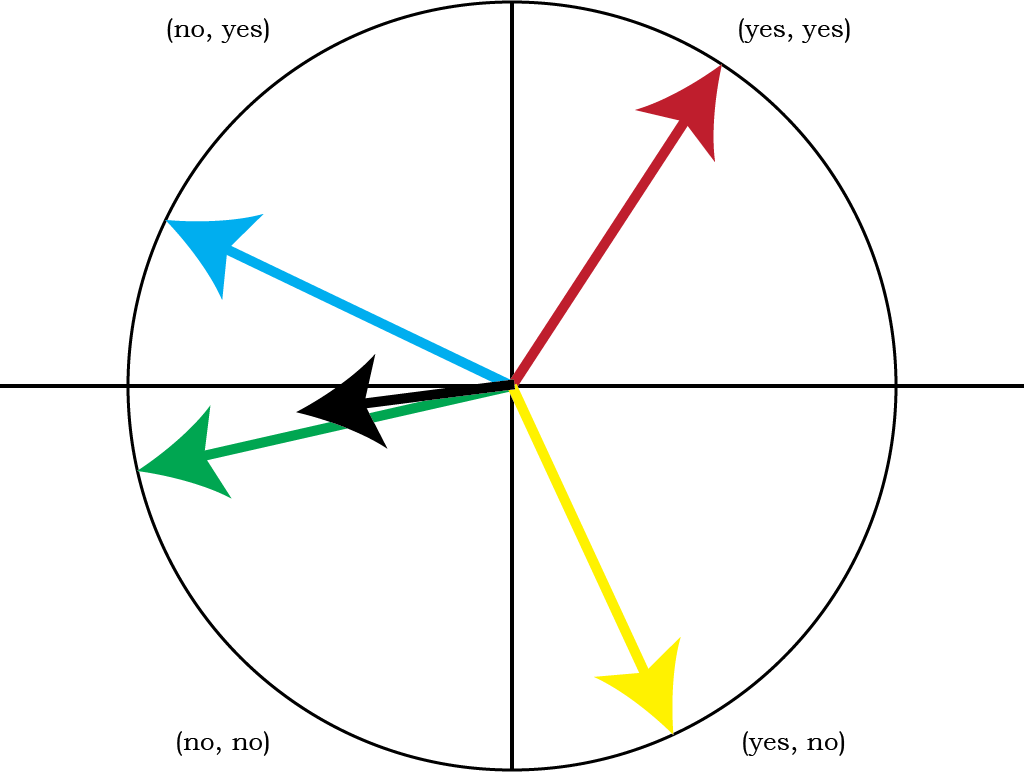
\includegraphics[width=0.45\textwidth]{figures/liquidfeedback2.png}
\caption{Liquid Feedback allows voters to cast their vote as a vector on a sphere, and the result (black) is calculated based on all the voters' vectors.}
\end{figure}

\subsection{Trust-based Recommendation Systems: An Axiomatic Approach}

The trust-based recommendations paper \cite{axioms} deals with the theory of recommendation systems, i.e. systems in which the end goal is to recommend new items for a user given her preferences and information about whose preferences she trusts.  The authors describe five axioms which may be desirable in trust-based recommendation systems:
\begin{enumerate}
	\item Symmetry (isomoorphic graphs result in isomorphic recommendations)
	\item Positive response (if a node with a netural recommendation is attached to a + voter, the recommendation moves from neutral to +)
	\item Independence of Irrelevant Stuff (a node's recommendation does not depend on nodes it cannot reach in the trust web)
	\item Neighborhood Consensus (if a nonvoters neighbors are all +, if that node votes + its neighbors recommendations do not change)
	\item Transitivity (the "trusts more" relationship is transitive)
\end{enumerate}
And they go on to prove that not all 5 are satisfiable within a single recommendation system, but that each subset of 4 uniquely leads to a recommendation system.  They suggest relaxations and replacements for axiom 5 which also lead to unique recommendation systems.  The authors offer a theoretical framework for the continued study of systems in which a user's preferences are inferred through explicit or implict trust relationships.

\section{Peer-to-peer Voting Scheme}

In designing our scheme we approached the issue from the other direction. We see voting as expressing the opinions of
people. When not everybody votes, the question is what are the opinions of non-voters and how can we include
these opinions in the final result. Currently, in commonly-used voting schemes their opinions are simply discarded.
We approached the issue from a machine learning perspective, seeing this as a prediction problem. We have a set
of known values (votes) and would like to infer the unknown values (non-voter opinions) from them. When deciding which data to
use we decided to use social network and trust relationships between people.  This is based on our anecdotal observations that
people tend to ask their friends how to vote when they themselves do not have a firm opinion on an issue. In our scheme,
we formalize this and make it explicit, thus simplifying and streamlining the process, making it scalable and
less time-consuming.

We decided to design a theoretical framework of a general process for inferring opinions from an entire population for
those who have not voted. How votes and inferred votes are tallied is not defined by our scheme, but for the
sake of discussion we assume that all votes are of equal weight and the final result is computed in the same manner as when
only cast votes are tallied.

In our scheme each member can delegate to an arbitrary number of other members, assigning each delegate an arbitrary fraction
of her total voting strength. Our scheme is orthogonal to the way in which members cast their vote. It can be a simple
yes/no or for/against decision, multiple option decision, or a ranking of options. All that is required is that votes have a
definite way to combine themselves from multiple delegates based on their ratios.

Our scheme is a two-stage process. In the first stage every member of a group chooses zero or more other members whom she
trusts and would delegate her voting decision to in the case she does not cast a vote herself. If she chooses nobody and
does not vote, her vote is discarded. If she chooses one or more delegates and does not vote, her vote is inferred from
her delegates in the chosen ratios. She can also declare that she wants part of her vote inferred from her delegates,
even if she does vote herself.

We present some examples. We have three members, Alice, Bob and Cathy. Alice can decide to delegate like this:
$$(\mathrm{Alice}, *)$$

This is a default which means her vote counts only if she casts a vote.
$$(\mathrm{Alice}, *), (\mathrm{Bob}, 0.4), (\mathrm{Cathy}, 0.6)$$

If Alice does not cast a vote, her vote is inferred $0.4$ from Bob and $0.6$ from Cathy. If she casts a vote, only her
vote counts.
$$(\mathrm{Alice}, 0.9), (\mathrm{Bob}, 0.04), (\mathrm{Cathy}, 0.06)$$

If she casts a vote then $0.9$ of her vote is counted, but still $0.04$ and $0.06$ is inferred from $B$ and $C$, respectively.
If she does not cast a vote, then her vote is inferred from Bob and Cathy in $0.4$ and $0.6$ shares.

These weighted delegation edges define a (social) network between members which is a kind of ``web of trust'' or
``trust network''. We can see it as a directed graph between (hopefully) everybody. We call this a ``delegation network''.

When a decision is needed, votes are cast. This is the second stage of the process. This is done in any manner settled on by the members and can be the same as in traditional voting. But, it is not required that everybody casts a vote and missing votes are not
simply discarded. For those who do not cast a vote, their vote is inferred. This is done transitively. So in the final example
above, if Bob does not cast a vote, then Bob's $0.4$ share of Alice's vote is inferred from Bob's own delegations. In the
case that none of Bob's delegates (transitively) casts a vote, then Alice's vote is wholly inferred from Cathy's vote.

This last possibility is an unfortunate one as it means we have lost the votes of Bob and all Bob's delegates who have not
voted, transitively. This is a very unlikely event (based on the six degrees of separation idea) and possible only if we allow
members to not choose any delegates (we could change the default delegation or make it compulsory for participants to delegate in the first phase).

\begin{figure}
\centering
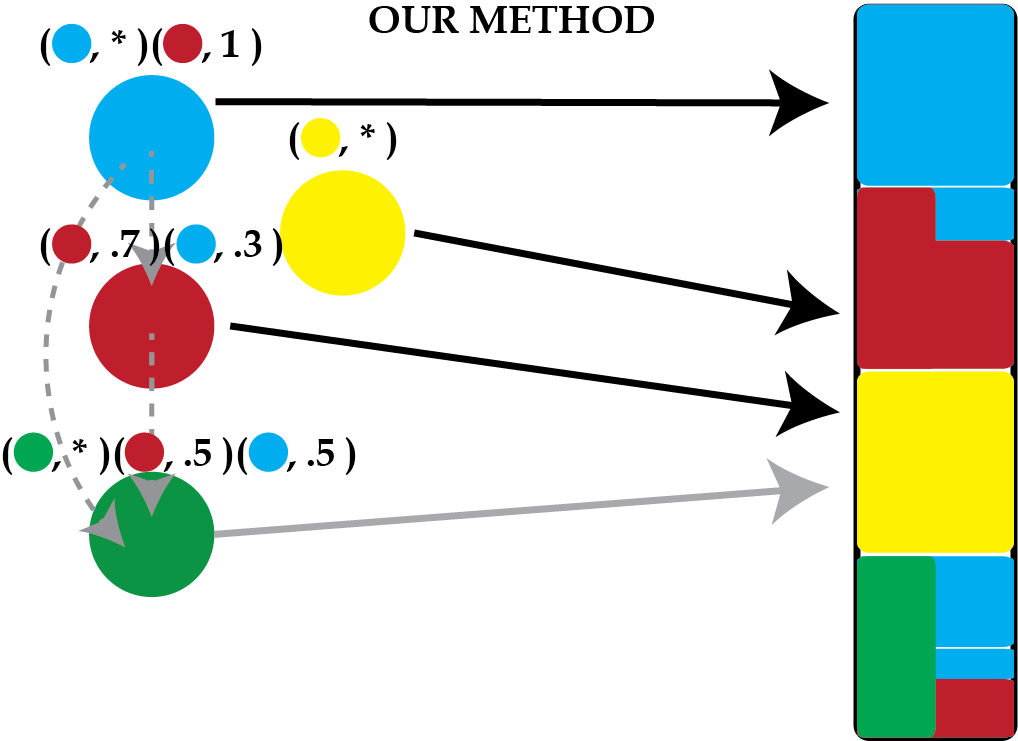
\includegraphics[width=0.45\textwidth]{figures/us3.png}
\caption{Our voting scheme allows precise definition of voting weight between delegates, and votes are counted recursively.}
\end{figure}

\section{Analysis}

Our scheme's definition is simple and general. From the point of view of the member she just has to (once) select delegates and ratios
between them, and then the scheme takes care of the rest. Depending on the use case of our scheme, members might have to define
multiple sets of delegates for various domains they are voting in.

``Casting a vote'' itself is not defined on purpose.  Our scheme deals only with a question of how to infer missing votes, thus augmenting
existing vote casting schemes.

In social choice theory, Arrow's impossibility theorem\cite{arrow} states limits on how ranked preferences of individuals are
converted into a community-wide (complete and transitive) ranking and this begs the question: how does this relate to our
scheme? We can observe that our scheme is orthogonal to this issue as it does not deal directly with the question of aggregating
the votes of individuals into a common decision, but just infers missing votes enabling any approach of aggregation to work
arguably better.  Ideally unsolvable conflicts such as those described by Arrow (in which $A > B, B > C, C > A$) could be resolved through the addition of iteration to our voting scheme, as in Liquid Democracy \cite{liquiddem}.

The additional data we gather in the first stage, the delegation network, allows us to infer missing votes in the second stage.
We implemented it as a graph-walking algorithm in Python. Code is available in the appendix.

Our scheme is inherently non-anonymous. We must know whose vote is whose so that uncast votes
can be inferred from the non-anonymous delegation network. The votes do not need to be public, but they still have to be stored non-anonymously.  (To assist voters in understanding why the loser lost and the winner won, the votes could be made public.  This allows voters to recalculate the results.) Moreover, a member's social network is revealed. This is a very private sort of
social network -- the network of influence between people. Such is additional limitation of our proposed scheme with respect to privacy.

\section{Future work}

Future research can address these privacy issues. For example, it would be possible to build a distributed system in which only people
one-hop away from the voter know how she cast her vote, but in further hops only an aggregate and anonymized vote is seen. Another
option is to develop some new cryptographic primitives which allow privacy on the one hand and verifiability on the other.
We do not really need to have public votes, just computability/verifiability of the results.

Additionally, an analysis of possible possible misuses of the scheme or issues with it should be performed. Can it be used by a
small number of members? Is it stable, or how much, in general, does the result change when one person changes her vote?

As we described, we see this is a general prediction problem of inferring of missing votes. It would be interesting to try
other existing (novel and traditional) approaches to predict missing data and use possible other sources of relevant data,
not just a trust network.

Someday, we would also like to convince Facebook that we are geniuses and that they should use their social network for the
power of good voting.  It may be possible to \emph{infer} voters' trust networks and link strengths based on their real social networks and the
interactions performed via applications like Facebook.  This would allow skipping the first stage of our scheme (in which voters
explicitly delegate their votes) while not endangering the voting power of any non-voters.

\bibliographystyle{abbrv}
\bibliography{references}

\onecolumn

\appendix
\section{Python implementation}

\vspace{1em}

\small
\lstinputlisting{voting.py}

\end{document}
